\documentclass[a4paper, 10pt, smallheadings, DIV15]{scrartcl}
\usepackage[utf8]{inputenc}
\usepackage{xspace}
\usepackage{hyphenat}
\usepackage{fancyvrb}
\newcommand{\rcm}[1]{\ensuremath{#1\;\mathrm{cm^{-1}}}\xspace}
\newcommand{\code}[1]{\nohyphens{\texttt{#1}}\xspace}
\usepackage{Sweave}
\begin{document}
\fvset{listparameters={\setlength{\topsep}{0pt}}}
\renewenvironment{Schunk}{\vspace{\topsep}}{\vspace{\topsep}}
{\center \sffamily \huge 
\textbf{Fitting Polynomial Baselines to Complete Spectra}\\[1ex] 
\large C.~Beleites,	DMRN, Università degli Studi di Trieste, Trieste/I\\[1ex] 
\today\\}

\subsection*{Syntax \& parameters} \code{spc.fit.poly.below (fit.to, apply.to = fit.to, 
poly.order = 1, npts.min = NULL, noise = 0,\\
short = NULL, user = NULL, date = NULL)}

\begin{labeling}{\code{poly.order}:~~~}
\item[\code{fit.to}:] \code{hyperSpec} object with the spectra whose baselines are to be fitted.
\item[\code{apply.to}:] \code{hyperSpec} object giving the spectral range, on wich the baselines should be evaluated.\\
 If \code{apply} is \code{NULL}, a \code{hyperSpec} object with the polynomial coefficients is returned 
 instead of evaluated baselines. 
\item[\code{poly.order}:] polynomial order of the baselines
\item[\code{npts.min}:] minimal number of data points per spectrum to be used for the fit.\\
\code{npts.min} defaults to the smaller of 3 times (\code{poly.order} + 1) or 
$\frac{1}{20th}$ of the number of data points per spectrum.\\
If \code{npts.min} $\leq$ \code{poly.order}, a warning is issued and \code{npts.min <- poly.order + 1} is used.   
 \item[\code{noise}:] a vector giving the amount of noise, see below. 
 \item[\code{short}, \code{user}, \code{date}:] are handed to \code{logentry}
 \end{labeling}

\subsection*{Specifying the spectral range}
\begin{figure}[b]
\begin{center}
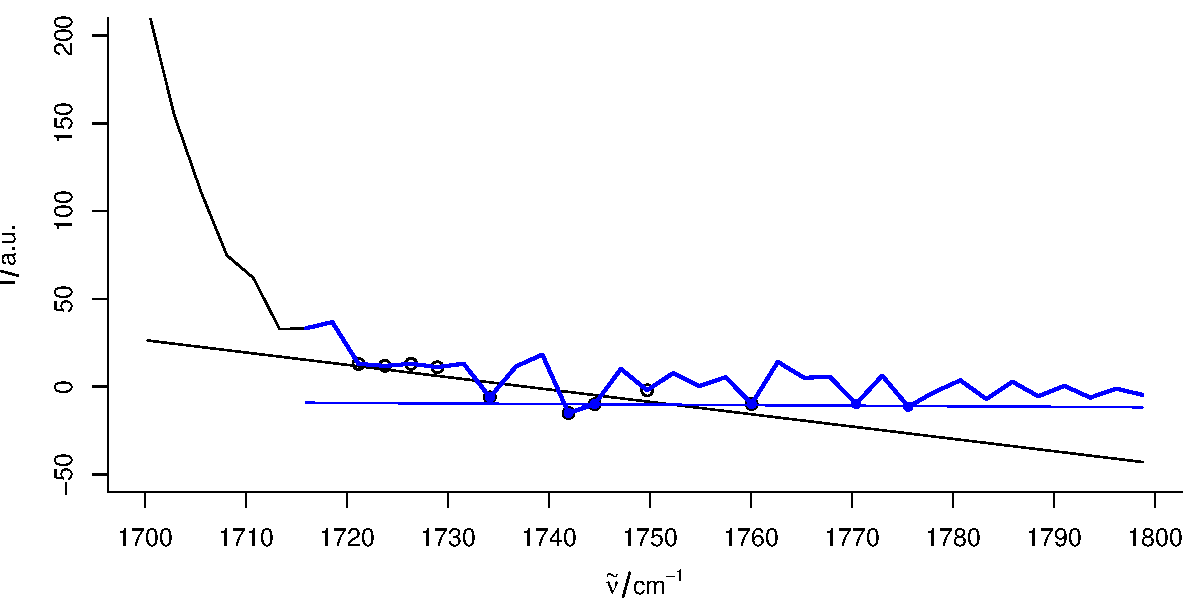
\includegraphics[width = .5\textwidth]{baselinebelow-figspcrange}
\caption{Influence of \code{fit.to} on the baseline polynomial. The black baseline is fit to the spectral range \rcm{1700 - 1800}, 
the blue to \rcm{1715 - 1800} only (dots \& circles: supporting points).}
\label{fig:spectralrange}
\end{center}
\end{figure}

The polynomials are always fit to \code{fit.to}, but are evaluated on the the wavelengths of \code{apply.to}. 
Therefore it is possible to exclude spectral regions that do not contribute to
the baseline from the fitting, while the baseline is used for the whole
spectrum.  
The choice of the spectral range in \code{fit.to} influences the resulting baselines to a certain extent, as becomes clear 
from figure~\ref{fig:spectralrange}.
Narrowing the spectral range in \code{fit.to} speeds up the fitting of the
polynomials:
\begin{Schunk}
\begin{Sinput}
> system.time(spc.fit.poly.below(chondro[], NULL, poly.order = 1, npts.min = 20, 
+     noise = 12))
\end{Sinput}
\begin{Soutput}
   user  system elapsed 
  3.352   0.008   3.364 
\end{Soutput}
\begin{Sinput}
> system.time(spc.fit.poly.below(chondro[, , -wl2i(chondro, 700:1700), index = TRUE], 
+     NULL, poly.order = 1, npts.min = 20, noise = 12))
\end{Sinput}
\begin{Soutput}
   user  system elapsed 
  2.000   0.008   2.009 
\end{Soutput}
\end{Schunk}

\subsection*{Fitting  polynomials of different orders}
\begin{figure}[t]
\begin{center}
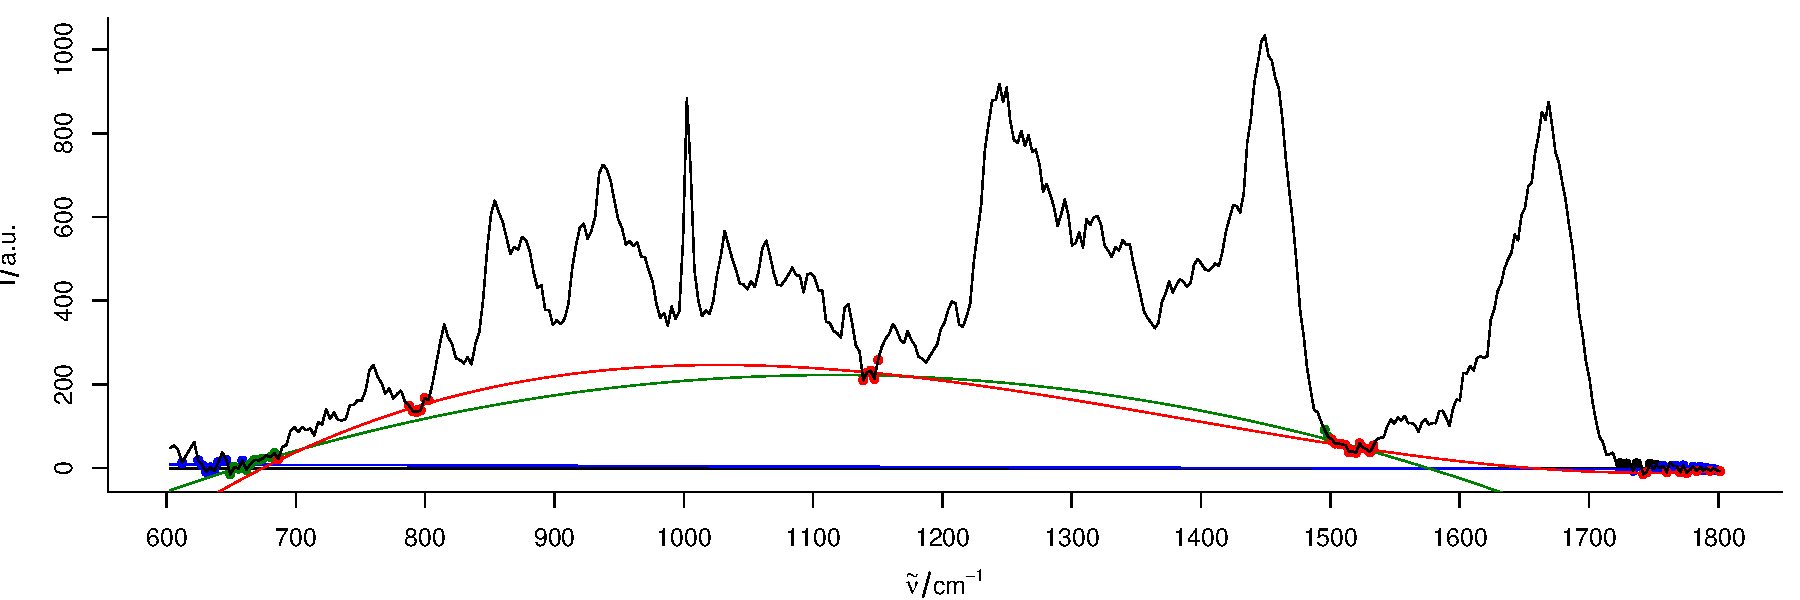
\includegraphics[width = .75\textwidth]{baselinebelow-figorder}
\caption{Baseline polynomial fit to the first spectrum of the chondro data set of order 
0 (black), 1 (blue), 2 (green), and 3 (red). The dots indicate the points used for the fitting of the polynomial.}
\label{fig:order}
\end{center}
\end{figure}
Figure~\ref{fig:order} shows the resulting baseline polynomial of 
\code{spc.fit.poly.below (chondro [1], poly.order = order)} 
with \code{order} $=$ 0 to 3 for the first spectrum of the chondro data set. 

\subsection*{The mecanism of fitting the baselines}
Appropriate spectral regions with supporting points for the baseline polynomials are calculated iteratively:
\begin{enumerate}
\item A polynomial of the requested order is fit to the considered spectral range.
\item Only the parts of the spectrum that lie below this polynomial plus the \code{noise} are retained as supporting points for 
the next iteration. 
\end{enumerate}
These two steps are repeated until either
\begin{itemize}
\item no further points are excluded, or
\item the next polynomial would have less than \code{npts.min} supporting points.
\end{itemize}
The baselines and respective supporting points for each iteration of
\code{spc.fit.poly.below (chondro [1], poly.order = 1)}
are shown in figure~\ref{fig:iter}.

\begin{figure}[bh]
\begin{center}
  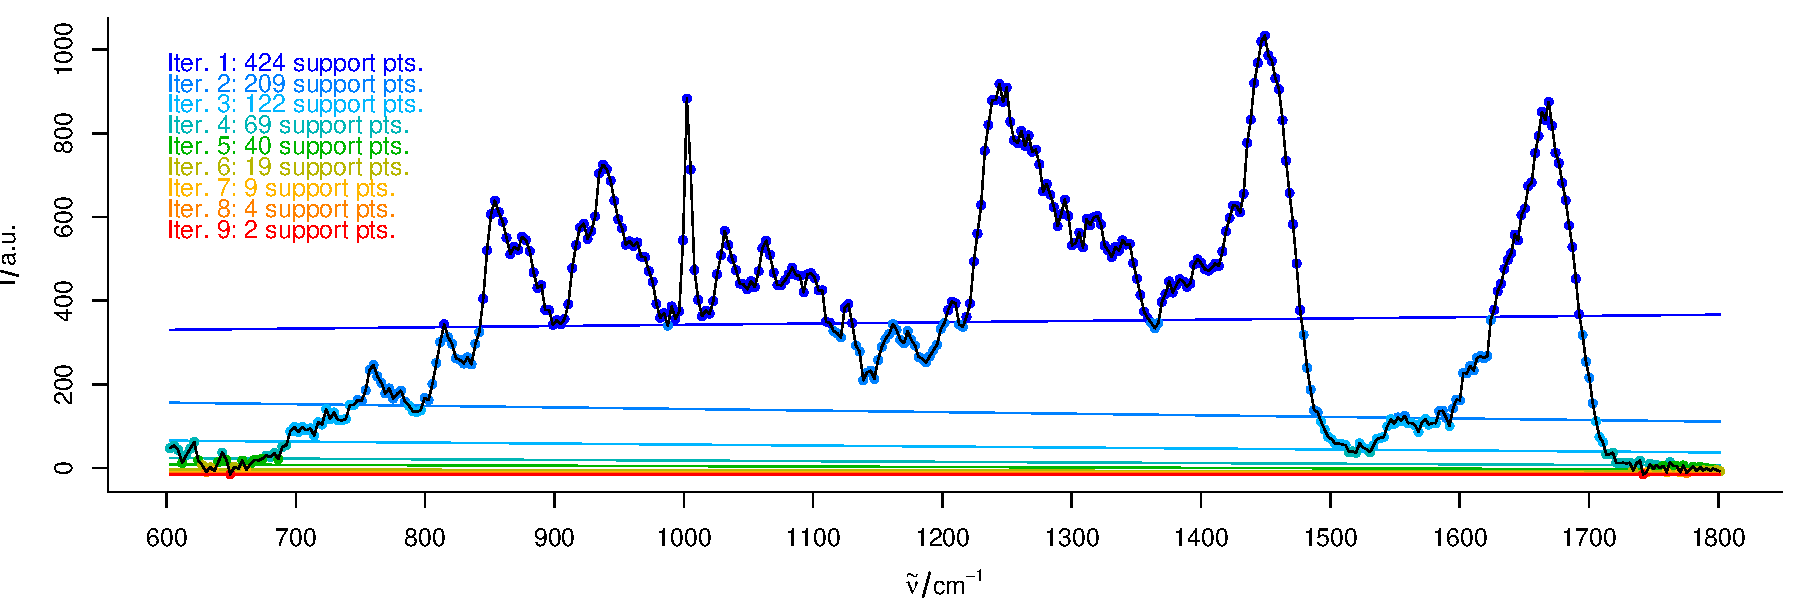
\includegraphics[width=.75\textwidth]{baselinebelow-fig1}
  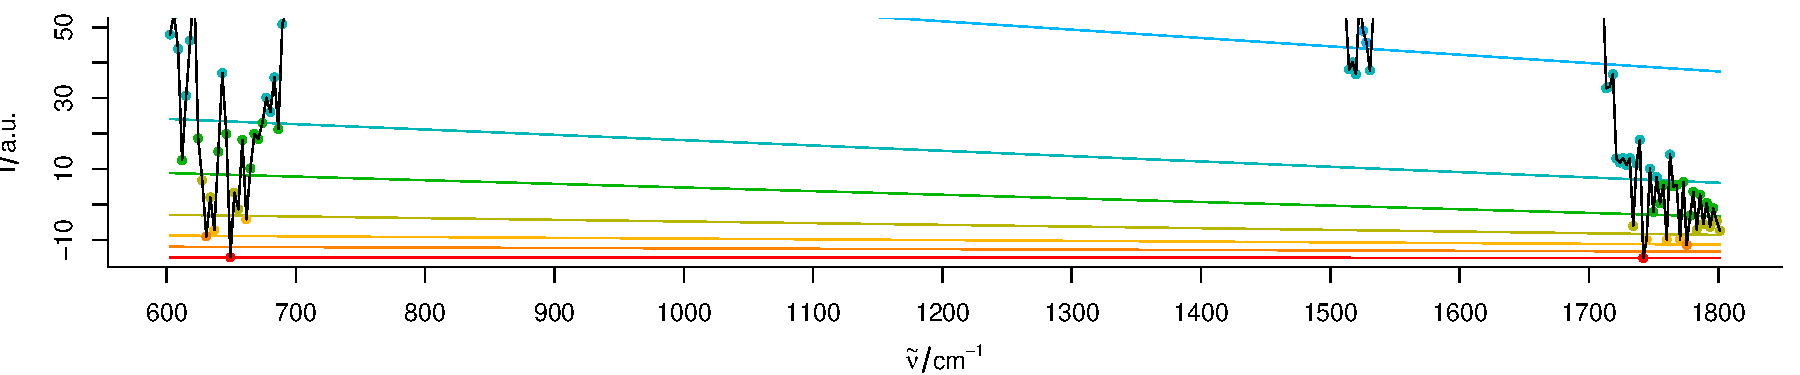
\includegraphics[width=.75\textwidth]{baselinebelow-fig2}
  \caption{Iterative fitting of the baseline. The dots give the supporting points for the baselines in the same color. 
  The lower part is a magnificaton of the intensity axis.}
  \label{fig:iter}
\end{center}
\end{figure}

\subsection*{The noise level}
\begin{figure}[t]
\begin{center}
  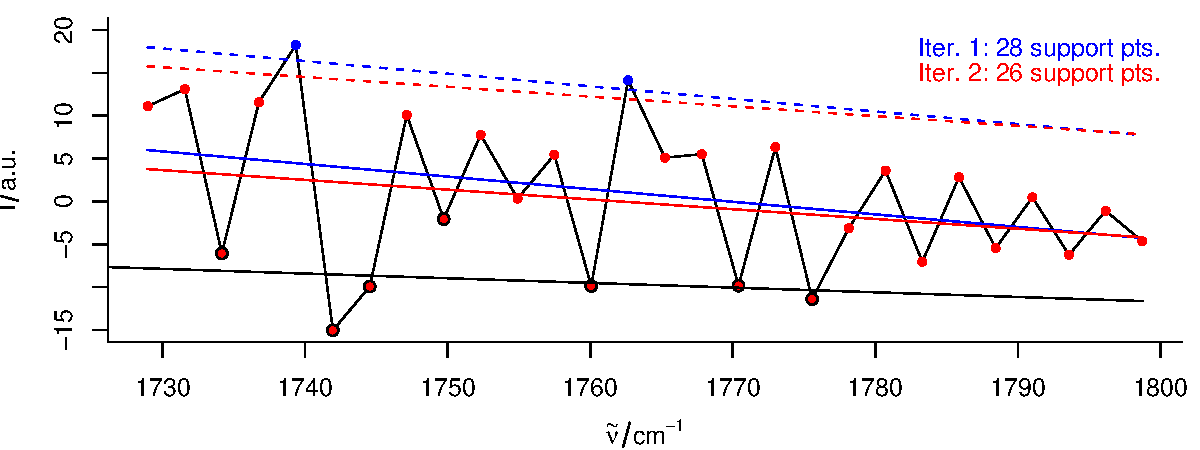
\includegraphics[width=.5\textwidth]{baselinebelow-fig3}
  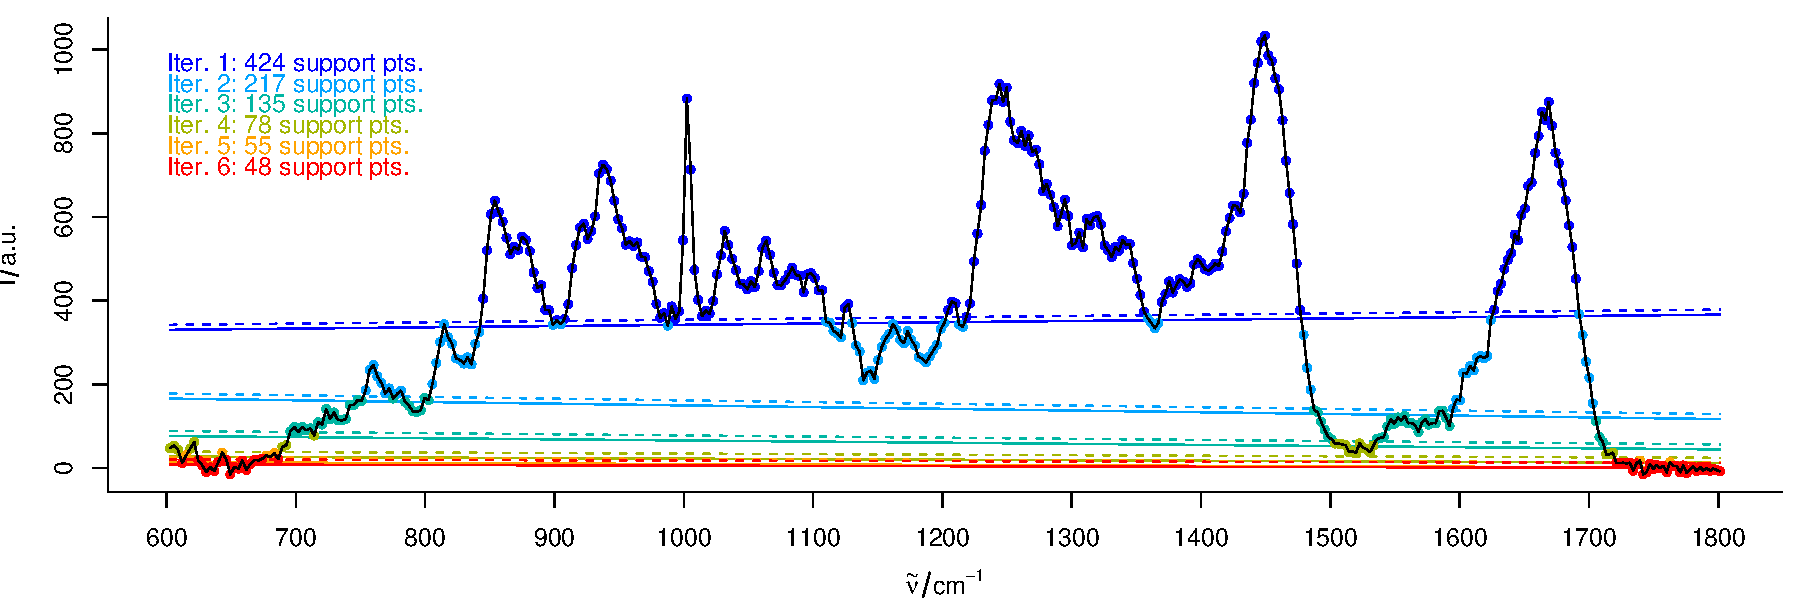
\includegraphics[width=.75\textwidth]{baselinebelow-fig4}
  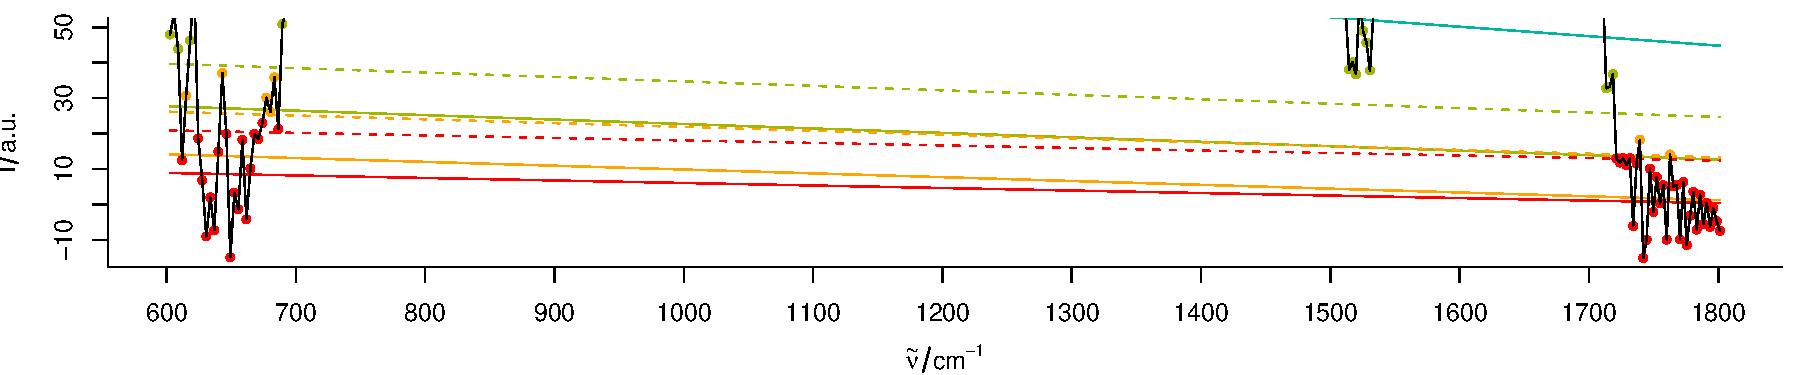
\includegraphics[width=.75\textwidth]{baselinebelow-fig5}
  \caption{Iterative fitting of the baseline with noise level. Upper part: effects of the noise parameter on the baseline 
  of a spectrum consisting only of noise and baseline:  without giving \code{noise} the resulting baseline 
  (black) is clearly too low. A noise level of 12 results in the red baseline. 
  The middle and lower part show the baseline fitting with noise level on the 
  complete spectrum.
  Color: iterations, dots/circles: supporting points for the respective baselines. Dashed: baseline plus noise. All points above this line are excuded from the next iteration.  
}
  \label{fig:noise}
\end{center}
\end{figure}

Besides defining a minimal number of supporting points, a ``noise level'' may be given.
Consider the spectral range above \rcm{1730} of the shown spectrum. The spectrum consists practically only of noise. 
The upper part of figure~\ref{fig:noise} illustrates the problem. As the baseline fitting algorithm cannot distinguish 
between noise and real bands appearing above the fitted polynomial, the resulting baseline (black) is too low if the \code{noise} 
parameter is not given.    

Setting the noise level to 12 (roughly 1.5 standard deviations), the fitting converges after 2 iteratons with a much better result. 
The resulting baselines for
\code{spc.fit.poly.below (chondro [1], poly.order = 1, noise = 12)}
of the whole spectrum are shown in the middle and lower part of figure~\ref{fig:noise} 

\code{noise} may be a single value for all spectra, or a vector with the noise level for each of the spectra separately.	
\end{document}
